\subsection{Ca sử dụng tra cứu du lịch}
\noindent Ca sử dụng này mô tả quá trình người dùng tìm kiếm thông tin về các địa điểm du lịch, sự kiện, hoặc các dịch vụ khác thông qua chức năng tìm kiếm của ứng dụng. Người dùng có thể nhập từ khóa và áp dụng các bộ lọc để thu hẹp kết quả. Bảng~\ref{tab:uc_search_spec} trình bày chi tiết đặc tả ca sử dụng, bao gồm luồng sự kiện chính, các điều kiện và yêu cầu liên quan. Các biểu đồ hoạt động, quan hệ (Bảng~\ref{tab:uc_search_diagrams}) và tuần tự (Hình~\ref{fig:3-3-5-sequence-diagram}) minh họa rõ hơn về quy trình và tương tác hệ thống khi người dùng thực hiện tra cứu.
% \vspace{0.5cm} % Adjust spacing if needed

% Use longtable environment
% Need \usepackage{longtable} and \usepackage{calc} in preamble
\begin{longtable}{| p{4cm} | p{\dimexpr\linewidth-4cm-4\tabcolsep} |} % Adjust widths as needed
    \caption{Đặc tả ca sử dụng tra cứu du lịch.} % Caption inside longtable
    \label{tab:uc_search_spec} \\ % Label after caption

    \hline
    \textbf{Mô tả} & Người dùng tra cứu và lọc tên địa điểm du lịch, sự kiện, điểm đến muốn tìm hiểu. \\
    \hline
    \endfirsthead % Header for the first page

    \hline
    % \multicolumn{2}{|c|}{(Tiếp theo)} \\ % Header for subsequent pages
    % \hline
    \textbf{Mô tả} & Người dùng tra cứu và lọc tên địa điểm du lịch, sự kiện, điểm đến muốn tìm hiểu. \\
    \hline
    \endhead

    \hline 
    % \multicolumn{2}{|r|}{{Tiếp tục ở trang sau}} \\ % Footer for pages before the last
    \endfoot

    \hline % Footer for the last page
    \endlastfoot

    % --- Table Content ---
    \textbf{Luồng cơ bản} & 1. Người dùng truy cập tab khám phá và bấm vào thanh tìm kiếm. \newline
                           2. Hệ thống hiển thị lịch sử tìm kiếm và các bộ lọc. \newline
                           3. Người dùng nhập từ khóa tìm kiếm. \newline
                           4. Người dùng chọn bộ lọc (sự kiện, địa điểm, nhà hàng, khách sạn, điểm đến, v.v.). \newline
                           5. Hệ thống tra cứu, lưu từ khóa tìm kiếm và hiển thị kết quả theo danh sách. \\
    \hline
    % \textbf{Luồng thay thế} & (Nếu có luồng thay thế, thêm vào đây) \\
    % \hline
    \textbf{Tiền điều kiện} & Người dùng đang đăng nhập và phiên đăng nhập chưa kết thúc. \\
    \hline
    \textbf{Hậu điều kiện} & - Người dùng có thể xem thông tin về các kết quả tìm kiếm.\newline
                           - Hệ thống lưu lại lịch sử tìm kiếm của người dùng. \newline
                           - Hệ thống có thể cập nhật sở thích của người dùng dựa trên từ khóa tìm kiếm. \\
    \hline
    \textbf{Yêu cầu phi chức năng} & Hệ thống xử lý tìm kiếm không quá 2 giây. \\
    % --- End Table Content ---

\end{longtable}
% \vspace{0.8cm}

\begin{table}[H] % Wrap the diagrams table
    \centering
    \caption{Biểu đồ hoạt động và quan hệ ca sử dụng tra cứu du lịch.} % Add caption
    \label{tab:uc_search_diagrams} % Add label
    \begin{tabular}{| c | c |}
        \hline
        \textbf{Biểu đồ hoạt động} & \textbf{Quan hệ} \\
        \hline
        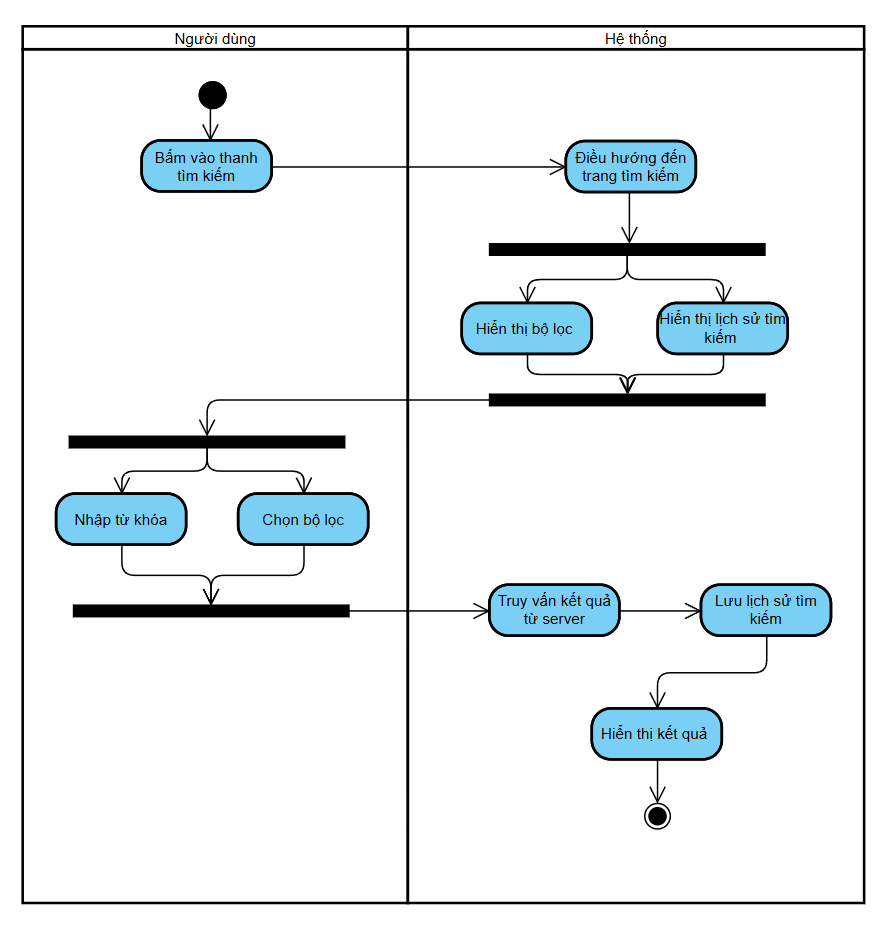
\includegraphics[width=0.5\linewidth]{figures/c3/3-3-5-ad.png}
        &
        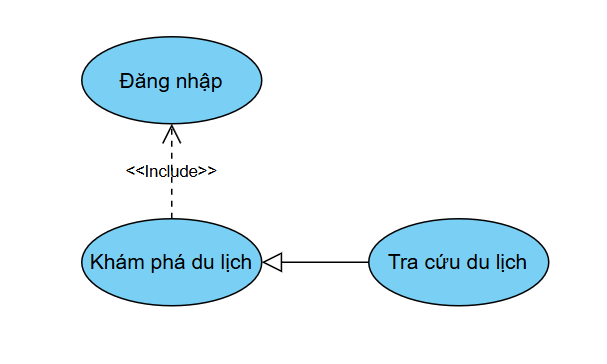
\includegraphics[width=0.45\linewidth]{figures/c3/3-3-5-rd.png} \\
        \hline
    \end{tabular}
\end{table}

\begin{figure}[H]
    \centering
    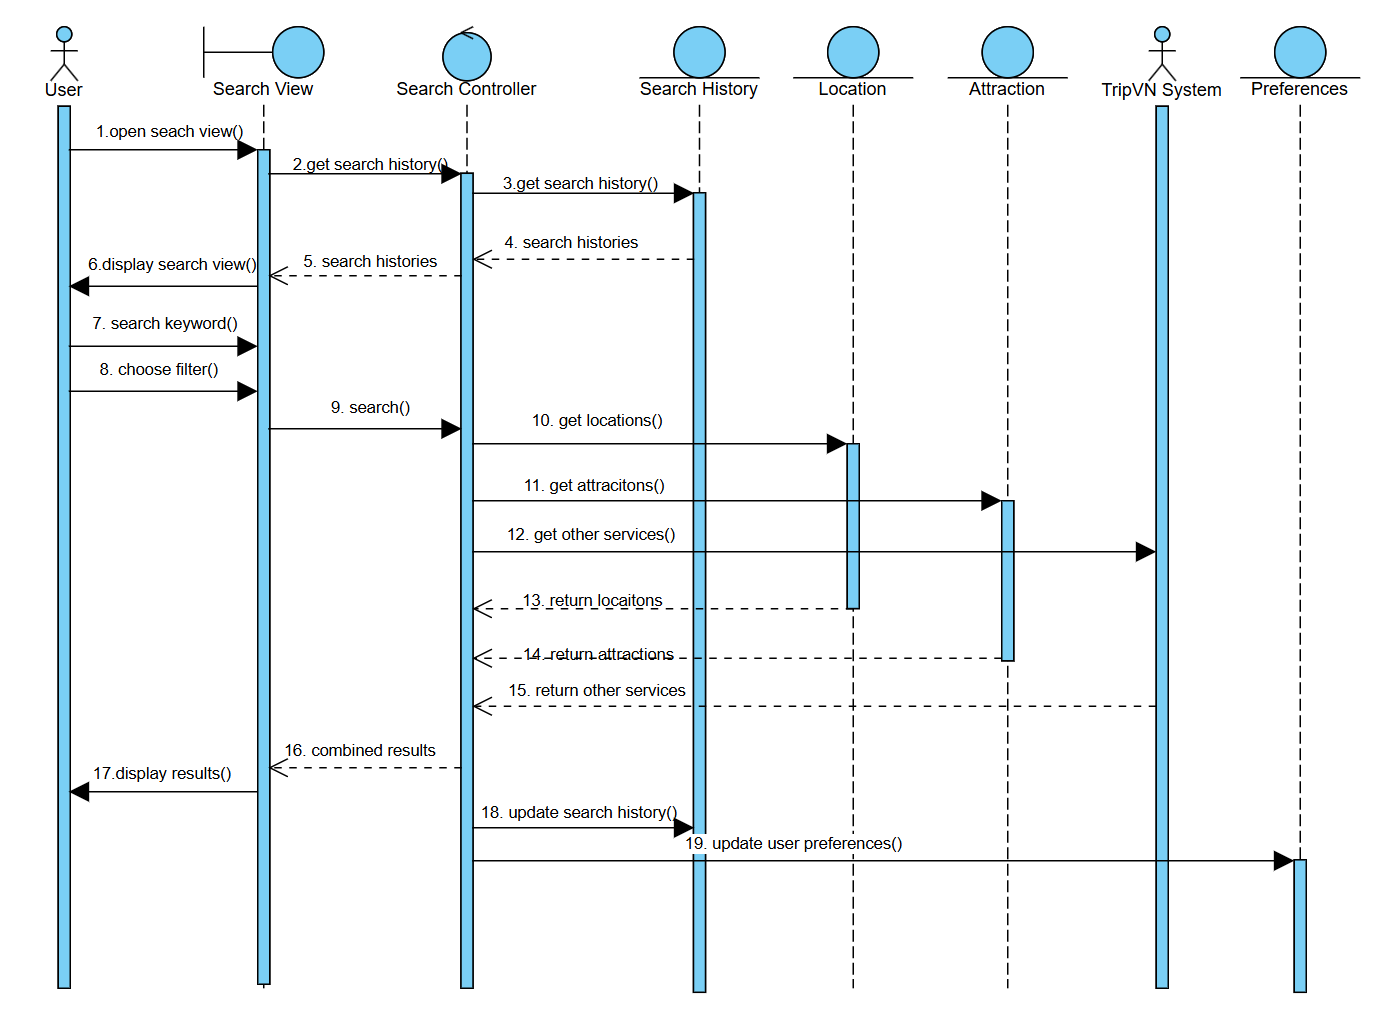
\includegraphics[width=1\textwidth]{figures/c3/3-3-5-sd.png} % Adjusted width slightly
    \caption{Biểu đồ tuần tự ca sử dụng tra cứu du lịch.}
    \label{fig:3-3-5-sequence-diagram}
\end{figure}